\section{Serial Com Windows}
	\subsection{Membuka Port}

		Dokumentasi SDK Platform menyatakan bahwa ketika membuka port komunikasi, panggilan ke CreateFile memiliki persyaratan berikut:

	

		\begin{enumerate} 
			
				\item  fdw Share Mode harus nol. Port komunikasi tidak dapat dibagikan dengan cara yang sama seperti file yang dibagikan. Aplikasi yang menggunakan TAPI dapat menggunakan fungsi TAPI untuk memfasilitasi berbagi sumber daya antar aplikasi. Untuk aplikasi yang tidak menggunakan TAPI, penanganan warisan atau duplikasi diperlukan untuk berbagi port komunikasi. Berurusan dengan duplikat berada di luar cakupan artikel ini, silakan merujuk ke dokumentasi Platform SDK untuk informasi lebih lanjut.
				\item  fdw Create harus menentukan bendera OPENEXISTING.
				\item  h Template File parameter harus NULL.

			\item Satu hal yang perlu diperhatikan tentang nama port adalah bahwa mereka secara tradisional telah COM1, COM2, COM3, atau COM4. Windows API tidak menyediakan mekanisme apa pun untuk menentukan port apa yang ada pada sistem. Beberapa sistem bahkan memiliki lebih banyak port daripada maksimum tradisional empat. Vendor perangkat keras dan pembuat perangkat serial-driver bebas memberi nama port apa pun yang mereka sukai. Untuk alasan ini, yang terbaik adalah pengguna memiliki kemampuan untuk menentukan nama port yang ingin mereka gunakan. Jika port tidak ada, kesalahan akan terjadi setelah mencoba membuka port, dan pengguna harus diberitahu bahwa port tidak tersedia.

			\item Satu hal yang perlu diperhatikan tentang nama port adalah bahwa mereka secara tradisional telah COM1, COM2, COM3, atau COM4. Windows API tidak menyediakan mekanisme apa pun untuk menentukan port apa yang ada pada sistem. Beberapa sistem bahkan memiliki lebih banyak port daripada maksimum tradisional empat. Vendor perangkat keras dan pembuat perangkat serial-driver bebas memberi nama port apa pun yang mereka sukai. Untuk alasan ini, yang terbaik adalah pengguna memiliki kemampuan untuk menentukan nama port yang ingin mereka gunakan. Jika port tidak ada, kesalahan akan terjadisetelah mencoba membuka port, dan pengguna harus diberitahu bahwa port tidak tersedia.

		\end{enumerate}
		
		\subsection{I atau O tumpang tindih}
		\begin{enumerate}
		

				\item I atau O yang tumpang tindih tidak sesederhana I atau O non-tumpang tindih, tetapi memungkinkan lebih banyak fleksibilitas dan efisiensi. Sebuah port terbuka untuk operasi tumpang tindih memungkinkan beberapa utas untuk melakukan operasi I atau O pada saat yang bersamaan dan melakukan pekerjaan lain ketika operasi sedang menunggu. Lebih jauh lagi, perilaku operasi yang tumpang tindih memungkinkan satu utas untuk mengeluarkan banyak permintaan yang berbeda dan bekerja di latar belakang sementara operasi masih menunggu.

				\item I atau O yang tumpang tindih tidak sesederhana I atau O non-tumpang tindih, tetapi memungkinkan lebih banyak fleksibilitas dan efisiensi. Sebuah port terbuka untuk operasi tumpang tindih memungkinkan beberapa utas untuk melakukan operasi I atau O pada saat yang bersamaan dan melakukan pekerjaan lain ketika operasi sedang menunggu. Lebih jauh lagi, perilaku operasi yang tumpang tindih memungkinkan satu utas untuk mengeluarkan banyak permintaan yang berbeda dan bekerja di latar belakang sementara operasi masih menunggu.


				\item Baik dalam aplikasi single-threaded maupun multithread, beberapa sinkronisasi harus dilakukan antara mengeluarkan permintaan dan memproses hasilnya. Satu utas harus diblokir sampai hasil operasi tersedia. Keuntungannya adalah I atau O yang tumpang tindih memungkinkan utas untuk melakukan beberapa pekerjaan antara waktu permintaan dan penyelesaiannya. Jika tidak ada pekerjaan yang dapat dilakukan, maka satu-satunya kasus untuk I atau O yang tumpang tindih adalah memungkinkan untuk respon pengguna yang lebih baik.

				\item I atau O yang tumpang tindih adalah jenis operasi yang digunakan sampel MTTTY. Ini menciptakan sebuah thread yang bertanggung jawab untuk membaca data port dan membaca status port. Ini juga melakukan pekerjaan latar belakang secara berkala. Program ini menciptakan untaian lain secara eksklusif untuk menulis data di luar port.
				
				\item Catatan Aplikasi terkadang menyalahgunakan sistem multithreading dengan membuat terlalu banyak utas. Meskipun menggunakan beberapa utas dapat menyelesaikan banyak masalah yang sulit, membuat untaian yang berlebihan bukanlah penggunaan yang paling efisien dalam aplikasi. Thread kurang regangan pada sistem daripada proses tetapi masih memerlukan sumber daya sistem seperti waktu CPU dan memori. Aplikasi yang menciptakan untaian berlebihan dapat mempengaruhi kinerja keseluruhan sistem.

		\end{enumerate}

	\begin{figure}[ht]
		\centerline{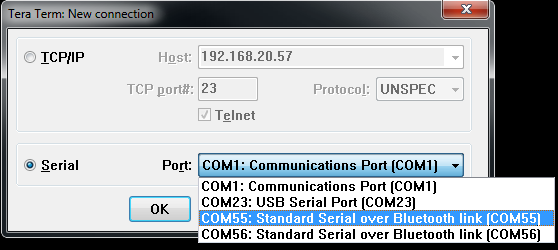
\includegraphics[width=1\textwidth]{figures/seria.png}}
		\caption{Serial Com Windows}
		\label{seria}
	\end{figure}
	Gambar \ref{seria} Contoh gambar.
		
		\begin{verbatim}
			HANDLE hComm;
			hComm = CreateFile( gszPort,  
                    GENERIC_READ | GENERIC_WRITE, 
                    0, 
                    0, 
                    OPEN_EXISTING,
                    FILE_FLAG_OVERLAPPED,
                    0);
			if (hComm == INVALID_HANDLE_VALUE)
				// error opening port; abort
		\end{verbatim}
	\subsection{Membaca dan menulis}
		\begin{enumerate}
			\item Membaca dari dan menulis ke port komunikasi di Windows sangat mirip dengan file input atau output  di Windows. Bahkan, fungsi yang melengkapi I atau O file adalah fungsi yang sama yang digunakan untuk serial I atau O. I atau O dapat dilakukan dengan salah satu dari dua cara: tumpang tindih atau tidak tumpang tindih. Dokumentasi SDK Platform menggunakan istilah asinkron dan sinkron untuk mengkonotasikan jenis operasi I atau O ini. Artikel ini, bagaimanapun, menggunakan istilah yang tumpang tindih dan tidak terabaikan.
			\item Nonoverlapped I atau O akrab bagi kebanyakan pengembang karena ini adalah bentuk tradisional I atau O, di mana operasi diminta dan diasumsikan lengkap ketika fungsi kembali. Dalam kasus I atau O yang tumpang tindih, sistem dapat kembali ke pemanggil segera bahkan ketika operasi tidak selesai dan akan memberi sinyal kepada pemanggil ketika operasi selesai. Program ini dapat menggunakan waktu antara permintaan I atau O dan penyelesaiannya untuk melakukan beberapa pekerjaan latar belakang.
		\end{enumerate}
				\subsubsection{Bacaan}
					\begin{enumerate}
						\item Fungsi ReadFile menerbitkan operasi baca. ReadFileEx juga mengeluarkan operasi baca, tetapi karena tidak tersedia pada Windows 95, itu tidak tercakup dalam artikel ini. Berikut adalah potongan kode yang merinci cara mempublikasikan permintaan baca. Perhatikan bahwa fungsi memanggil fungsi untuk memproses data jika ReadFile mengembalikan TRUE. Ini adalah fungsi yang sama yang disebut jika operasi menjadi tumpang tindih. Perhatikan flag fWaitingOnRead yang didefinisikan oleh kode; ini menunjukkan apakah operasi baca tumpang tindih atau tidak. Ini digunakan untuk mencegah penciptaan operasi baca baru jika mereka luar biasa.
					\end{enumerate}
				
				\begin{verbatim}
				DWORD dwRead;
					BOOL fWaitingOnRead = FALSE;
					OVERLAPPED osReader = {0};

						// Create the overlapped event. Must be closed before exiting
						// to avoid a handle leak.
						osReader.hEvent = CreateEvent(NULL, TRUE, FALSE, NULL);

						if (osReader.hEvent == NULL)
						// Error creating overlapped event; abort.

						if (!fWaitingOnRead) {
						// Issue read operation.
						if (!ReadFile(hComm, lpBuf, READ_BUF_SIZE, &dwRead, &osReader)) {
						if (GetLastError() != ERROR_IO_PENDING)     // read not delayed?
						// Error in communications; report it.
					else
						fWaitingOnRead = TRUE;
				}
					else {    
						// read completed immediately
						HandleASuccessfulRead(lpBuf, dwRead);
			}
		}
				\end{verbatim}

				\begin{enumerate}
						\item Bagian kedua dari operasi yang tumpang tindih adalah deteksi penyelesaiannya. Pegangan acara dalam struktur OVERLAPPED diteruskan ke fungsi WaitForSingleObject, yang akan menunggu hingga objek diberi isyarat. Setelah acara ditandai, operasi selesai. Ini tidak berarti bahwa itu berhasil diselesaikan, hanya saja itu selesai. Fungsi GetOverlappedResult melaporkan hasil operasi. Jika kesalahan terjadi, GetOverlappedResult mengembalikan FALSE dan GetLastError mengembalikan kode kesalahan. Jika operasi selesai dengan sukses, GetOverlappedResult akan mengembalikan TRUE.

						
						\item Catatan Get Overlapped Result dapat mendeteksi penyelesaian operasi, serta mengembalikan status kegagalan operasi. Get Overlapped Result mengembalikan FALSE dan Get Last Error mengembalikan ketika operasi tidak selesai. Selain itu, Get Overlapped Result dapat dibuat untuk memblokir hingga operasi selesai. Ini secara efektif mengubah operasi yang tumpang tindih menjadi operasi non-tumpang tindih dan dicapai dengan melewatkan TRUE sebagai parameter bWait.
				\end{enumerate}


			
		
			\subsubsection{Penulisan}
				\begin{enumerate}
					\item Pengarsipan data dari port komunikasi sangat mirip dengan membaca, karena menggunakan banyak API yang sama. Cuplikan kode di bawah ini menunjukkan cara menghapus dan menunggu operasi tulis selesai.
				\end{enumerate}
				\begin{verbatim}
				BOOL WriteABuffer(char * lpBuf, DWORD dwToWrite)
{
   OVERLAPPED osWrite = {0};
   DWORD dwWritten;
   DWORD dwRes;
   BOOL fRes;

   // Create this write operation's OVERLAPPED structure's hEvent.
   osWrite.hEvent = CreateEvent(NULL, TRUE, FALSE, NULL);
   if (osWrite.hEvent == NULL)
      // error creating overlapped event handle
      return FALSE;

   // Issue write.
   if (!WriteFile(hComm, lpBuf, dwToWrite, &dwWritten, &osWrite)) {
      if (GetLastError() != ERROR_IO_PENDING) { 
         // WriteFile failed, but isn't delayed. Report error and abort.
         fRes = FALSE;
      }
      else
         // Write is pending.
         dwRes = WaitForSingleObject(osWrite.hEvent, INFINITE);
         switch(dwRes)
         {
            // OVERLAPPED structure's event has been signaled. 
            case WAIT_OBJECT_0:
                 if (!GetOverlappedResult(hComm, &osWrite, &dwWritten, FALSE))
                       fRes = FALSE;
                 else
                  // Write operation completed successfully.
                  fRes = TRUE;
                 break;
            
            default:
                 // An error has occurred in WaitForSingleObject.
                 // This usually indicates a problem with the
                // OVERLAPPED structure's event handle.
                 fRes = FALSE;
                 break;
         }
      }
   }
   else
      // WriteFile completed immediately.
      fRes = TRUE;

   CloseHandle(osWrite.hEvent);
   return fRes;
}
\end{verbatim}	

	\subsection{Serial Status}
		\begin{enumerate}
			\item Ada dua metode untuk mengambil status port komunikasi. Yang pertama adalah dengan mengatur event mask yang menyebabkan pemberitahuan aplikasi ketika peristiwa yang diinginkan terjadi. Fungsi Set Comm Mask mengatur masker kejadian ini, dan fungsi Wait Comm Event menunggu kejadian yang diinginkan terjadi. Metode kedua untuk mengambil status port komunikasi adalah secara berkala memanggil beberapa fungsi status yang berbeda. Polling, tentu saja, tidak efisien dan tidak direkomendasikan.
		\end{enumerate}
			\subsection{Communications Events}
				\begin{enumerate}
				\item Komunikasi dapat terjadi kapan saja selama menggunakan port komunikasi. Dua langkah yang terlibat dalam menerima pemberitahuan acara komunikasi adalah sebagai berikut:

				\item Set Comm Mask menetapkan peristiwa yang diinginkan yang menyebabkan pemberitahuan.
			\item WaitCommEvent menerbitkan pemeriksaan status. Pemeriksaan status dapat berupa operasi tumpang-tindih atau non-tumpang tindih, seperti halnya operasi baca dan tulis.
				\item Catatan : Peristiwa kata dalam konteks ini merujuk pada acara komunikasi saja. Itu tidak mengacu pada objek peristiwa yang digunakan untuk sinkronisasi.


				\end{enumerate}
			
	\begin{verbatim}
	DWORD dwStoredFlags;

	dwStoredFlags = EV_BREAK | EV_CTS   | EV_DSR | EV_ERR | EV_RING |\
                EV_RLSD | EV_RXCHAR | EV_RXFLAG | EV_TXEMPTY ;
		if (!SetCommMask(hComm, dwStoredFlags))
   // error setting communications mask
	\end{verbatim}
\subsection{Flow Control}
	\begin{enumerate}
		\item Kontrol aliran dalam komunikasi serial menyediakan mekanisme untuk menangguhkan komunikasi sementara salah satu perangkat sibuk atau karena alasan tertentu tidak dapat melakukan komunikasi apa pun. Secara tradisional ada dua jenis kontrol aliran: perangkat keras dan perangkat lunak.

\item Masalah umum dengan komunikasi serial adalah operasi tulis yang sebenarnya tidak menulis data ke perangkat. Seringkali, masalah terletak pada kontrol aliran yang digunakan ketika program tidak menentukannya. Pemeriksaan dekat dari struktur DCB mengungkapkan bahwa satu atau lebih dari anggota berikut mungkin BENAR: fOutxCtsFlow, fOutxDsrFlow, atau fOutX. Mekanisme lain untuk mengungkapkan bahwa kontrol aliran diaktifkan adalah memanggil ClearCommError dan memeriksa struktur COMSTAT. Ini akan mengungkapkan ketika transmisi ditangguhkan karena kontrol aliran.

\item Sebelum membahas jenis-jenis pengendalian aliran, pemahaman yang baik tentang beberapa istilah sudah teratur. Komunikasi serial terjadi antara dua perangkat. Secara tradisional, ada PC dan modem atau printer. PC diberi label Data Terminal Equipment . DTE kadang-kadang disebut tuan rumah. Modem, printer, atau peralatan periferal lainnya diidentifikasi sebagai Peralatan Komunikasi Data . DCE kadang-kadang disebut sebagai perangkat.
\end{enumerate}

\cite{bai2004windows}
\cite{carvey2005tracking}
\cite{boling2003programming}			
